\documentclass[border=6pt]{standalone}
\usepackage{tikz}
\usepackage{pgfplots}
\pgfplotsset{compat=1.18}
\usetikzlibrary{arrows.meta,positioning,shapes.geometric,fit,backgrounds,calc,decorations.pathreplacing,patterns}
\usetikzlibrary{pgfplots.groupplots}
\tikzset{
  blk/.style={rectangle, rounded corners=2pt, draw=black!70, thick, fill=blue!6,
              minimum height=8mm, minimum width=20mm, align=center, font=\small},
  io/.style={rectangle, rounded corners=6pt, draw=black!70, thick, fill=green!8,
             minimum height=8mm, align=center, font=\small},
  proc/.style={rectangle, draw=black!70, thick, fill=orange!10, minimum height=8mm,
               align=center, font=\small},
  dec/.style={diamond, aspect=2, draw=black!70, thick, fill=yellow!15, align=center, font=\footnotesize},
  warnbox/.style={rectangle, rounded corners=2pt, draw=red!60!black, thick, fill=red!7,
                  minimum height=8mm, align=center, font=\small},
  oklbox/.style={rectangle, rounded corners=2pt, draw=green!45!black, thick, fill=green!8,
                 minimum height=8mm, align=center, font=\small},
  ar/.style={-{Latex[length=2mm]}, thick},
  arl/.style={-{Latex[length=2mm]}, thick, dashed, draw=black!55},
  lbl/.style={font=\footnotesize\itshape, text=black!60},
}
\definecolor{good}{RGB}{34,139,34}
\definecolor{bad}{RGB}{178,34,34}
\definecolor{warn}{RGB}{218,165,32}
\definecolor{pesblue}{RGB}{0,45,98}
\definecolor{complete}{RGB}{30,125,79}
\definecolor{partial}{RGB}{176,106,0}
\definecolor{blocked}{RGB}{166,43,43}
% --- figure-local styles -------------------------------------------------
\tikzset{
  phdr/.style={rectangle, rounded corners=2pt, draw=pesblue, thick, fill=pesblue,
               text=white, font=\small\bfseries, inner sep=3pt,
               text width=6.8cm, align=center},
  pvary/.style={rectangle, rounded corners=2pt, draw=complete!75!black, thick,
                fill=complete!9, font=\footnotesize, inner sep=3.5pt,
                text width=6.8cm, align=left},
  pfix/.style={rectangle, rounded corners=2pt, draw=black!45, thick, fill=black!7,
               font=\scriptsize, text=black!68, inner sep=3.5pt,
               text width=6.8cm, align=left},
  pres/.style={rectangle, rounded corners=1pt, draw=black!30, fill=black!3,
               font=\scriptsize\itshape, text=black!75, inner sep=3pt,
               text width=6.8cm, align=left},
  tagvary/.style={font=\scriptsize\bfseries, text=complete!70!black},
  tagfix/.style={font=\scriptsize\bfseries, text=black!55},
}
\begin{document}
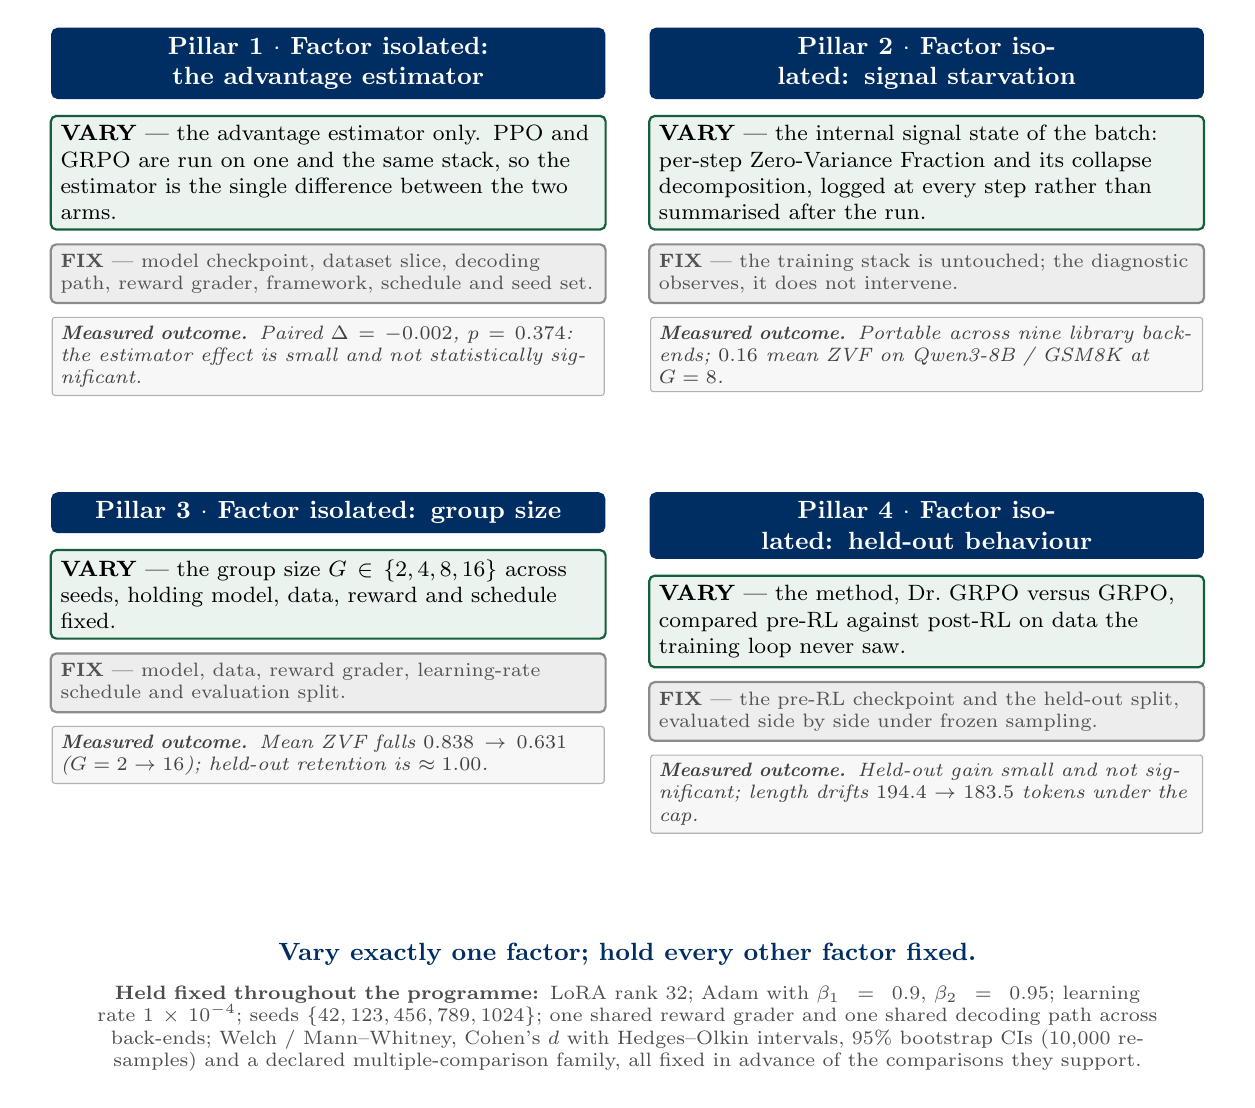
\begin{tikzpicture}

% ============================ four pillars ==============================
\foreach \i/\hdr/\vary/\fix/\res in {%
1/{Pillar 1 $\cdot$ Factor isolated: the advantage estimator}%
 /{\textbf{VARY} --- the advantage estimator only. PPO and GRPO are run on one and the same stack, so the estimator is the single difference between the two arms.}%
 /{\textbf{FIX} --- model checkpoint, dataset slice, decoding path, reward grader, framework, schedule and seed set.}%
 /{Paired $\Delta = -0.002$, $p = 0.374$: the estimator effect is small and not statistically significant.},%
2/{Pillar 2 $\cdot$ Factor isolated: signal starvation}%
 /{\textbf{VARY} --- the internal signal state of the batch: per-step Zero-Variance Fraction and its collapse decomposition, logged at every step rather than summarised after the run.}%
 /{\textbf{FIX} --- the training stack is untouched; the diagnostic observes, it does not intervene.}%
 /{Portable across nine library back-ends; $0.16$ mean ZVF on Qwen3-8B / GSM8K at $G=8$.},%
3/{Pillar 3 $\cdot$ Factor isolated: group size}%
 /{\textbf{VARY} --- the group size $G \in \{2,4,8,16\}$ across seeds, holding model, data, reward and schedule fixed.}%
 /{\textbf{FIX} --- model, data, reward grader, learning-rate schedule and evaluation split.}%
 /{Mean ZVF falls $0.838 \to 0.631$ ($G=2 \to 16$); held-out retention is $\approx 1.00$.},%
4/{Pillar 4 $\cdot$ Factor isolated: held-out behaviour}%
 /{\textbf{VARY} --- the method, Dr.~GRPO versus GRPO, compared pre-RL against post-RL on data the training loop never saw.}%
 /{\textbf{FIX} --- the pre-RL checkpoint and the held-out split, evaluated side by side under frozen sampling.}%
 /{Held-out gain small and not significant; length drifts $194.4 \to 183.5$ tokens under the cap.}%
}
{
  \pgfmathsetmacro{\px}{mod(\i-1,2)*7.6}
  \pgfmathsetmacro{\py}{-int((\i-1)/2)*5.9}
  \node[phdr, anchor=north] (h\i) at (\px,\py) {\hdr};
  \node[pvary, below=2.0mm of h\i] (v\i) {\vary};
  \node[pfix, below=1.6mm of v\i]   (f\i) {\fix};
  \node[pres, below=1.6mm of f\i]   (r\i) {\textbf{Measured outcome.} \res};
}

% ============================ spine banner =============================
\node[anchor=north, font=\small\bfseries, text=pesblue] at (3.8,-11.5)
  {Vary exactly one factor; hold every other factor fixed.};
\node[anchor=north, font=\scriptsize, text=black!70, text width=15.0cm, align=center]
  at (3.8,-12.05)
  {\textbf{Held fixed throughout the programme:} LoRA rank $32$; Adam with
   $\beta_1=0.9$, $\beta_2=0.95$; learning rate $1\times10^{-4}$; seeds
   $\{42,123,456,789,1024\}$; one shared reward grader and one shared decoding
   path across back-ends; Welch / Mann--Whitney, Cohen's $d$ with Hedges--Olkin
   intervals, $95\%$ bootstrap CIs ($10{,}000$ resamples) and a declared
   multiple-comparison family, all fixed in advance of the comparisons they support.};

\end{tikzpicture}
\end{document}
